\documentclass{article}
\usepackage[utf8]{inputenc}
\usepackage{xcolor}
\usepackage{graphicx}
\usepackage{float}
\usepackage{minted}
\usepackage{circuitikz}
\usepackage{tikz}
\usetikzlibrary{shapes, arrows, calc, positioning, circuits.logic.US, circuits.logic.IEC}
\usepackage{geometry}
\geometry{a4paper, margin=1in}
\usepackage{hyperref}
\usemintedstyle{trac}

\usepackage{fancyhdr}
\pagestyle{fancy}
\fancyhf{}
\renewcommand{\headrulewidth}{0pt}
\fancyfoot[C]{\small 010153101 Digital Circuit and Microprocessor Fundamental \\ Semester 2/2025}
\fancyfoot[R]{\thepage}

% Redefine plain style to match fancy style (for the title page)
\fancypagestyle{plain}{%
  \fancyhf{}%
  \fancyfoot[C]{\small 010153101 Digital Circuit and Microprocessor Fundamental \\ Semester 2/2025}%
  \fancyfoot[R]{\thepage}%
  \renewcommand{\headrulewidth}{0pt}%
}

\title{Laboratory Exercise 6 - Week 2 \\ Registers and Applications}
\author{}
\date{}

\begin{document}

\maketitle

The purpose of this exercise is to investigate latches, flip-flops, and registers. This second week focuses on advanced storage elements and their applications.

\setcounter{figure}{6}

\section*{Part IV}

Figure 7 shows a circuit with three different storage elements: a gated D latch, a positive-edge triggered D flip-flop, and a negative-edge triggered D flip-flop.

\begin{figure}[H]
    \centering
    % Placeholder for Figure 7: Three storage elements
    \begin{circuitikz}
    \ctikzset{logic ports=ieee}
    \ctikzset{flipflops/scale=1}

    % Define Styles
    % Latch: Transparent high (no clock wedge)
    \tikzset{latch/.style={flipflop, flipflop def={t1=D, t3=Clk, t6=Q}}} 
    % Pos-Edge FF: Standard D FF with clock wedge
    \tikzset{pos-ff/.style={flipflop D, flipflop def={t6=Q}}}
    % Neg-Edge FF: Standard D FF with clock wedge and negation
    \tikzset{neg-ff/.style={flipflop D, flipflop def={t6=Q, n3=1}}}

    % Nodes
    % 1. Gated D Latch
    \node[latch] (latch) at (0, 0) {};
    \node[above] at (latch.north) {Gated D Latch};

    % 2. Pos-Edge D FF
    \node[pos-ff] (pos_ff) at (0, -3.5) {};
    \node[above] at (pos_ff.north) {Pos-Edge D FF};

    % 3. Neg-Edge D FF
    \node[neg-ff] (neg_ff) at (0, -7) {};
    \node[above] at (neg_ff.north) {Neg-Edge D FF};

    % Inputs aligned to latch
    % D connected to Latch Pin 1 (D)
    % Clock connected to Latch Pin 3 (Clk)
    \coordinate (D_pin) at (latch.pin 1);
    \coordinate (Clk_pin) at (latch.pin 3);
    
    \draw (D_pin) -- ++(-3, 0) node[left] (D_in) {D};
    \draw (Clk_pin) -- ++(-3, 0) node[left] (Clk_in) {Clock};

    % Bus Lines
    % Vertical bus for D
    \coordinate (D_bus_top) at ($(D_in.east) + (0.5, 0)$);
    \draw (D_bus_top) |- (pos_ff.pin 1);
    \draw (D_bus_top) |- (neg_ff.pin 1);
    \draw (D_bus_top) -- (D_pin); % Connect to latch D
    \fill[black] (D_bus_top) circle (2pt);
    \fill[black] (D_bus_top |- pos_ff.pin 1) circle (2pt);

    % Vertical bus for Clock
    \coordinate (Clk_bus_top) at ($(Clk_in.east) + (1.0, 0)$);
    \draw (Clk_bus_top) |- (pos_ff.pin 3);
    \draw (Clk_bus_top) |- (neg_ff.pin 3);
    \draw (Clk_bus_top) -- (Clk_pin); % Connect to latch Clk
    \fill[black] (Clk_bus_top) circle (2pt);
    \fill[black] (Clk_bus_top |- pos_ff.pin 3) circle (2pt);

    % Outputs
    \draw (latch.pin 6) -- ++(1, 0) node[right] {$Q_a$};
    \draw (pos_ff.pin 6) -- ++(1, 0) node[right] {$Q_b$};
    \draw (neg_ff.pin 6) -- ++(1, 0) node[right] {$Q_c$};

\end{circuitikz}

    \caption{Circuit for Part IV.}
    \label{fig:three_storage}
\end{figure}

\begin{figure}[H]
    \centering
    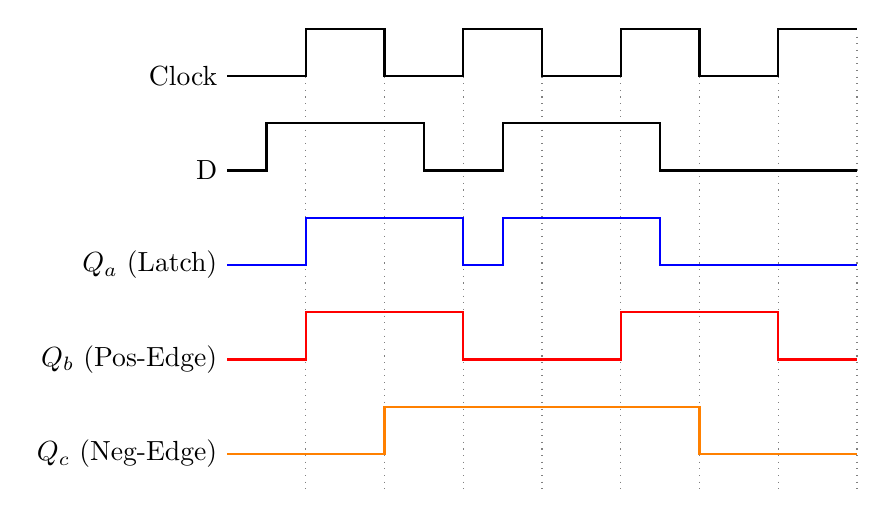
\begin{tikzpicture}
    % Define coordinates
    \def\tick{0.2}
    \def\h{0.6} % Height of logic high
    \def\sep{-1.2} % Separation between signals

    % Labels
    \node[anchor=east] at (0, 0) {Clock};
    \node[anchor=east] at (0, \sep) {D};
    \node[anchor=east] at (0, 2*\sep) {$Q_a$ (Latch)};
    \node[anchor=east] at (0, 3*\sep) {$Q_b$ (Pos-Edge)};
    \node[anchor=east] at (0, 4*\sep) {$Q_c$ (Neg-Edge)};

    % Draw Axes/Grid lines
    \foreach \x in {1,2,...,8} {
        \draw[dotted, gray] (\x, 0.5) -- (\x, 4*\sep - 0.5);
    }

    % Clock Signal (Period = 2 units)
    % 0-1 Low, 1-2 High...
    \draw[thick] (0,0) -- (1,0) -- (1,\h) -- (2,\h) -- (2,0) -- (3,0) -- (3,\h) -- (4,\h) -- (4,0) -- (5,0) -- (5,\h) -- (6,\h) -- (6,0) -- (7,0) -- (7,\h) -- (8,\h);

    % D Input (Arbitrary)
    % 0-0.5: 0
    % 0.5-2.5: 1
    % 2.5-3.5: 0
    % 3.5-5.5: 1
    % 5.5-8.0: 0
    \draw[thick] (0, \sep) -- (0.5, \sep) -- (0.5, \sep+\h) -- (2.5, \sep+\h) -- (2.5, \sep) -- (3.5, \sep) -- (3.5, \sep+\h) -- (5.5, \sep+\h) -- (5.5, \sep) -- (8, \sep);

    % Qa (Gated D Latch) - Transparent when Clk=1
    \draw[thick, blue] (0, 2*\sep) 
        -- (1, 2*\sep)       % Hold 0
        -- (1, 2*\sep+\h)    % @1.0 Clk->1, D=1 -> 1
        -- (3, 2*\sep+\h)    % Hold 1 until 3.0
        -- (3, 2*\sep)       % @3.0 become 0
        -- (3.5, 2*\sep)     % Follow 0
        -- (3.5, 2*\sep+\h)  % @3.5 D->1, Clk=1 -> Follow 1
        -- (5.5, 2*\sep+\h)  % Hold/Follow 1
        -- (5.5, 2*\sep)     % @5.5 Follow 0
        -- (8, 2*\sep);      % 0

    % Qb (Pos-Edge D FF) - Sample D at Rising Edge (1, 3, 5, 7)
    \draw[thick, red] (0, 3*\sep) 
        -- (1, 3*\sep)    % Init 0
        -- (1, 3*\sep+\h) % @1 D=1 -> 1
        -- (3, 3*\sep+\h) % Hold
        -- (3, 3*\sep)    % @3 D=0 -> 0
        -- (5, 3*\sep)    % Hold
        -- (5, 3*\sep+\h) % @5 D=1 -> 1
        -- (7, 3*\sep+\h) % Hold
        -- (7, 3*\sep)    % @7 D=0 -> 0
        -- (8, 3*\sep);

    % Qc (Neg-Edge D FF) - Sample D at Falling Edge (2, 4, 6)
    \draw[thick, orange] (0, 4*\sep) 
        -- (2, 4*\sep)    % Init 0
        -- (2, 4*\sep+\h) % @2 D=1 -> 1
        -- (6, 4*\sep+\h) % Hold
        -- (6, 4*\sep)    % @6 D=0 -> 0
        -- (8, 4*\sep);

\end{tikzpicture}

    \caption{Waveforms for Part IV.}
    \label{fig:three_storage_timing}
\end{figure}

Implement and simulate this circuit using the Quartus software as follows:
\begin{enumerate}
    \item Create a new Quartus project.
    \item \textbf{First, implement the circuit using Schematic Design.} Draw the circuit using the Block Editor.
    \item Compile the schematic design and perform a functional simulation to verify its correctness.
    \item \textbf{Next, implement the circuit using Structural VHDL Design.}
    \item Write a VHDL file that instantiates the three storage elements. For this part you should no longer use the KEEP directive.
    \item Compile your code and use the Technology Map Viewer to examine the implemented circuit. Verify that the latch uses one lookup table and that the flip-flops are implemented using the flip-flops provided in the target FPGA.
    \item Create a Vector Waveform File (.vwf) that specifies the inputs and outputs of the circuit. Draw the inputs D and Clock as indicated in Figure 7. Use functional simulation to obtain the three output signals. Observe the different behavior of the three storage elements.
\end{enumerate}

\begin{figure}[H]
    \centering
    \begin{minted}[frame=single, fontsize=\small, linenos]{vhdl}
LIBRARY ieee;
USE ieee.std_logic_1164.all;

ENTITY d_latch IS
    PORT ( D, Clk : IN STD_LOGIC;
           Q : OUT STD_LOGIC);
END d_latch;

ARCHITECTURE Behavior OF d_latch IS
BEGIN
    PROCESS ( D, Clk )
    BEGIN
        IF Clk = '1' THEN
            Q <= D;
        END IF;
    END PROCESS;
END Behavior;

LIBRARY ieee;
USE ieee.std_logic_1164.all;

ENTITY pos_edge_d_ff IS
    PORT ( D, Clk : IN STD_LOGIC;
           Q : OUT STD_LOGIC);
END pos_edge_d_ff;

ARCHITECTURE Behavior OF pos_edge_d_ff IS
BEGIN
    PROCESS ( Clk )
    BEGIN
        IF RISING_EDGE(Clk) THEN
            Q <= D;
        END IF;
    END PROCESS;
END Behavior;

LIBRARY ieee;
USE ieee.std_logic_1164.all;

ENTITY neg_edge_d_ff IS
    PORT ( D, Clk : IN STD_LOGIC;
           Q : OUT STD_LOGIC);
END neg_edge_d_ff;

ARCHITECTURE Behavior OF neg_edge_d_ff IS
BEGIN
    PROCESS ( Clk )
    BEGIN
        IF FALLING_EDGE(Clk) THEN
            Q <= D;
        END IF;
    END PROCESS;
END Behavior;
    \end{minted}
    \caption{VHDL code for the D latch and D flip-flops.}
    \label{fig:vhdl_storage}
\end{figure}

\section*{Part V}

We wish to display the hexadecimal value of an 8-bit number A on the two 7-segment displays HEX3-2. We also wish to display the hex value of an 8-bit number B on the two 7-segment displays HEX1-0. The values of A and B are inputs to the circuit which are provided by means of switches SW7-0. To input the values of A and B, first set the switches to the desired value of A, store these switch values in a register, and then change the switches to the desired value of B. Finally, use an adder to generate the arithmetic sum S = A + B, and display this sum on the 7-segment displays HEX5-4. Show the carry-out produced by the adder on LEDR(0).

\begin{figure}[H]
    \centering
    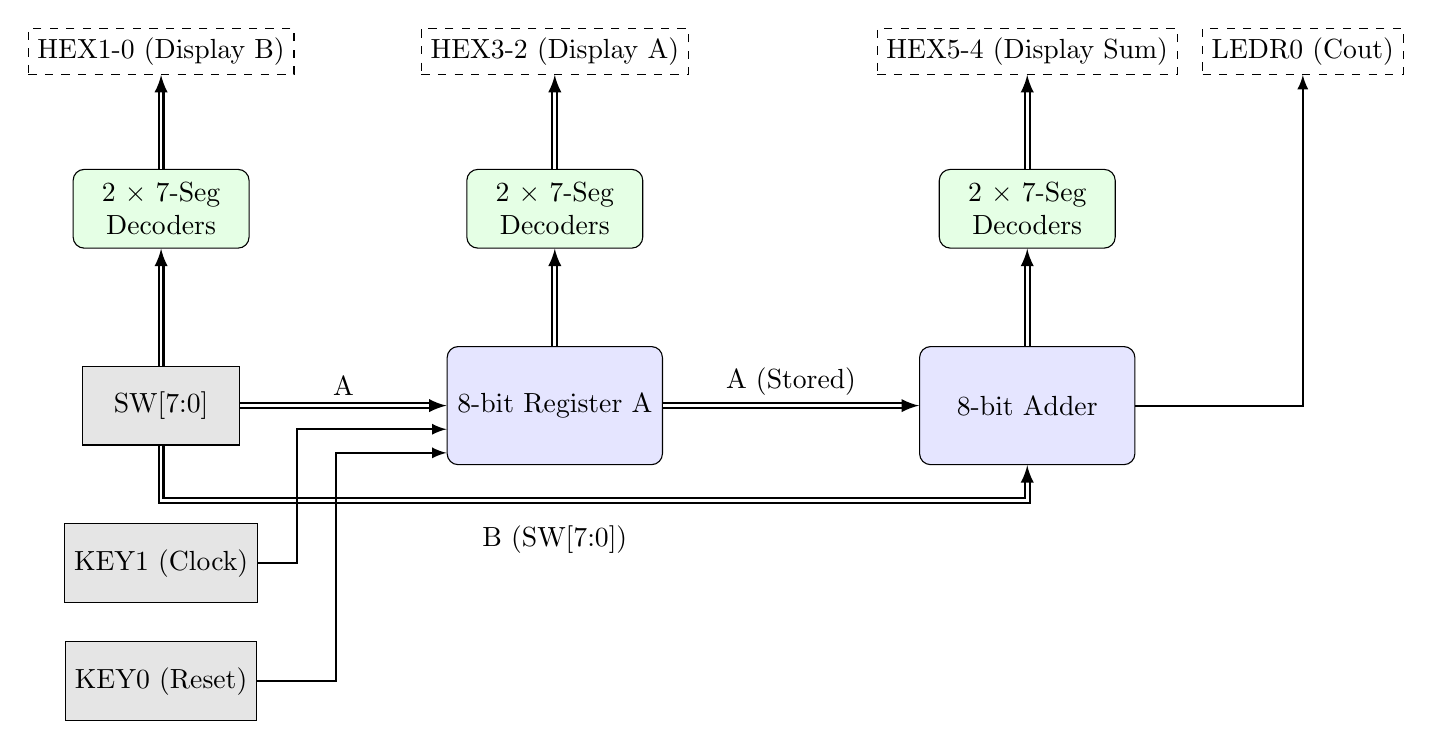
\begin{tikzpicture}[
    auto,
    node distance=2.5cm,
    block/.style={rectangle, draw, fill=blue!10, text width=2.5cm, text centered, rounded corners, minimum height=1.5cm},
    decoder/.style={rectangle, draw, fill=green!10, text width=2cm, text centered, rounded corners, minimum height=1cm},
    line/.style={draw, -latex, thick},
    bus/.style={draw, -latex, thick, double, double distance=1pt}
]

    % Nodes
    % Inputs on the left
    \node (sw) [draw, rectangle, fill=gray!20, minimum width=2cm, minimum height=1cm] {SW[7:0]};
    \node [draw, rectangle, fill=gray!20, minimum width=2cm, minimum height=1cm, below of=sw, node distance=2cm] (key1) {KEY1 (Clock)};
    \node [draw, rectangle, fill=gray!20, minimum width=2cm, minimum height=1cm, below of=key1, node distance=1.5cm] (key0) {KEY0 (Reset)};
    
    % Main Data Path - Increased distances
    \node [block, right of=sw, node distance=5cm] (reg) {8-bit Register A};
    \node [block, right of=reg, node distance=6cm] (adder) {8-bit Adder};
    
    % Decoders
    \node [decoder, above of=reg, node distance=2.5cm] (decA) {2 $\times$ 7-Seg Decoders};
    \node [decoder, above of=sw, node distance=2.5cm] (decB) {2 $\times$ 7-Seg Decoders};
    \node [decoder, above of=adder, node distance=2.5cm] (decSum) {2 $\times$ 7-Seg Decoders};

    % Displays (represented as groups) - Increased vertical distance
    \node [draw, rectangle, dashed, above of=decA, node distance=2cm] (hexA) {HEX3-2 (Display A)};
    \node [draw, rectangle, dashed, above of=decB, node distance=2cm] (hexB) {HEX1-0 (Display B)};
    \node [draw, rectangle, dashed, above of=decSum, node distance=2cm] (hexSum) {HEX5-4 (Display Sum)};
    \node [draw, rectangle, dashed, right of=hexSum, node distance=3.5cm] (led) {LEDR0 (Cout)};

    % Connections
    % SW to Register
    \draw [bus] (sw) -- node {A} (reg);
    
    % SW to Adder (B input) - Needs to bypass Register
    % Route under the register with clear clearance
    \draw [bus] (sw.south) -- ++(0, -0.7) coordinate (bypass) -- (bypass -| adder.south) -- (adder.south);
    \node at (bypass -| reg) [below=0.2cm] {B (SW[7:0])};

    % Register to Adder
    \draw [bus] (reg) -- node {A (Stored)} (adder);
    
    % Register to Decoder A to Display A
    \draw [bus] (reg.north) -- (decA.south);
    \draw [bus] (decA.north) -- (hexA.south);
    
    % SW to Decoder B to Display B
    \draw [bus] (sw.north) -- (decB.south);
    \draw [bus] (decB.north) -- (hexB.south);
    
    % Adder to Decoder Sum to Display Sum
    \draw [bus] (adder.north) -- (decSum.south);
    \draw [bus] (decSum.north) -- (hexSum.south);
    
    % Adder to LED
    \draw [line] (adder.east) -| (led.south);

    % Control connections
    % Route from left side inputs to Register
    \draw [line] (key1.east) -- ++(0.5, 0) |- ($(reg.west) + (0, -0.3)$);
    \draw [line] (key0.east) -- ++(1.0, 0) |- ($(reg.west) + (0, -0.6)$); % Reset to bottom of register

\end{tikzpicture}

    \caption{Block diagram for Part V.}
    \label{fig:part5_block_diagram}
\end{figure}

\begin{figure}[H]
    \centering
    \begin{minted}[frame=single, fontsize=\small, linenos]{vhdl}
LIBRARY ieee;
USE ieee.std_logic_1164.all;

ENTITY reg8 IS
    PORT ( D : IN STD_LOGIC_VECTOR(7 DOWNTO 0);
           Resetn, Clock : IN STD_LOGIC;
           Q : OUT STD_LOGIC_VECTOR(7 DOWNTO 0));
END reg8;

ARCHITECTURE Behavior OF reg8 IS
BEGIN
    PROCESS ( Resetn, Clock )
    BEGIN
        IF Resetn = '0' THEN
            Q <= (OTHERS => '0');
        ELSIF RISING_EDGE(Clock) THEN
            Q <= D;
        END IF;
    END PROCESS;
END Behavior;
    \end{minted}
    \caption{VHDL code for an 8-bit register with asynchronous reset.}
    \label{fig:vhdl_reg8}
\end{figure}

\begin{enumerate}
    \item Create a new Quartus project which will be used to implement the desired circuit on your DE0-CV board.
    \item \textbf{Implement the circuit using Structural VHDL Design.} Write a VHDL file that provides the necessary functionality. Use KEY0 as an active-low asynchronous reset, and use KEY1 as a clock input.
    \item Include the necessary pin assignments for the pushbutton switches and 7-segment displays, and then compile the circuit.
    \item Download the circuit onto your DE0-CV board and test its functionality by toggling the switches and observing the output displays.
\end{enumerate}

\vspace{1cm}
\noindent \textbf{Updated By:} R. Sutthaweekul \\
\textbf{Release Date:} 2026-01-01

\end{document}
